\documentclass[12pt]{report}

\usepackage{palatino}
\usepackage{hyperref}
\usepackage{upquote}
\usepackage{graphicx}
\usepackage[margin=1in]{geometry}
\renewcommand{\baselinestretch}{1.5}

\begin{document}

\title{Alshayun: A mobile education application}
\author{Jacob Chappell}
\date{\today}
\maketitle

\tableofcontents
\listoffigures

% Definitions in bold: \textbf{}

\chapter{Introduction}

    \section{What is Alshayun?}

\textbf{Alshayun} is a mobile application for delivering articles consisting of
rich text and interactive \textbf{applet}s to \textbf{reader}s. Written in the
portable \textbf{Ionic} framework, \textbf{Alshayun} is capable of running on
the Web, Android devices, and Apple iOS devices. However, \textbf{Alshayun} has
currently only been tested on a Samsung Galaxy S7 device running Android.

\textbf{Alshayun} is designed with three actors in mind: the \textbf{content
author}, the \textbf{reader}, and the \textbf{developer}. The \textbf{content
author} is anyone who has anything they would like to write about, potentially
making use of interactive and embedded \textbf{applet}s as assistive visual
aids. The \textbf{reader} is anyone who would like to read what one or more
\textbf{content author}s have to say. The \textbf{developer} is the one capable of
developing \textbf{applet}s and other functionality of \textbf{Alshayun} of
which \textbf{content author}s and \textbf{reader}s can make use. Note that
while I speak of these roles in the singular, many individuals may inhabit any
given role, and some individuals may inhabit multiple roles.

    \section{Inspiration}

After taking a numerical methods course as part of my Computer Science
undergraduate degree, I became fascinated with Bézier curves. Whilst researching
Bézier curves online, I came across an article titled \textit{A Primer on Bézier
Curves} \cite{pomax} authored by someone named Pomax. The highly detailed and
enlightening article was filled with interactive \textbf{applet}s designed to
strengthen the \textbf{reader}'s understanding of each progressively difficult
concept.

Intrigued by Pomax's work, I was inspired to develop a sort of content delivery
mechanism designed to allow \textbf{content author}s like Pomax author similar
articles and deliver them to interested \textbf{reader}s. Supporting the
development and use of interesting, interactive \textbf{applet}s was a priority.
I recognized that any such modern application needed to be mobile-friendly, and
so I decided to develop exclusively with mobility in mind.

    \section{About the Name}

\textbf{Alshayun} was originally meant to be tailored towards mathematics
education.  However, during the process of developing the application, I
realized that I had created a much more generalizable platform capable of
servicing any subject and perhaps more. Albeit, I decided to keep the name I
gave the application from the time of its inception---a name that carries with
it certain mathematical connotations.

Algebra (from the Arabic ``al-jabr'') is one of the most powerful mathematical
devices and fields of study, as well as my personal favorite subject of
mathematics. The English-speaking world inherited its written algebraic works
from Latin, which came from Spanish, which came from Arabic. This line of
inheritance spanned many years and involved merchants and trade routes, among
other things. In the original Arabic sources, the word ``al-shayun,'' meaning
``the unknown thing,'' was frequently used to describe the unknown in algebraic
equations. Therefore, I found ``al-shayun'' to be an appropriate name filled
with mathematical historical meaning.

To learn more about how ``al-shayun'' came to be the letter ``x'' used in modern
algebra, check out the article \textit{Why X marks the unknown} by Terry Moore
\cite{moore}.

\chapter{Technologies Used}

    \section{Node.js}

\textbf{Node\@.js (Node)} \cite{nodejs} is a \textbf{JavaScript} runtime
designed mainly to facilitate writing scalable, server-side software in
\textbf{JavaScript}. Before \textbf{Node}, first released in May of 2009, the
idea of writing server-side software in \textbf{JavaScript} was relatively
unknown. Since its conception, \textbf{Node} has received much attention and
both praise and criticism from \textbf{developer}s.

Less than a year after \textbf{Node}'s inception, a package manager was released
in January of 2010 named the \textbf{Node Package Manager (NPM)} \cite{npm}.
\textbf{NPM} has since played a vital role in the development of most
\textbf{JavaScript} software and frameworks and has transcended its original
intent to become a general JavaScript package manager.

While developing \textbf{Alshayun}, I never interacted directly with
\textbf{Node.} However, \textbf{NPM} was a vital part of my development process.
It is for that reason that I mention \textbf{NPM} and \textbf{Node} as a used
technology.

    \section{TypeScript}

\textbf{TypeScript} \cite{typescript} is a superset of \textbf{JavaScript} that
ultimately compiles into \textbf{JavaScript}. \textbf{TypeScript} complements
\textbf{JavaScript} with type safety and true object-oriented programming
constructs such as classes, access modifiers, and inheritance. In
\textbf{TypeScript}, every variable and symbol in general will have a type,
either stated explicitly by the programmer or inferred by the
\textbf{TypeScript} compiler from usage. The \textbf{TypeScript} compiler is
available for installation as an \textbf{NPM} package.

As the programming language of \textbf{Alshayun}, \textbf{TypeScript} has been
extraordinarily useful in development. In particular, the access to
object-oriented programming constructs has allowed me to write clean, modular,
and purpose-driven code.

    \section{Angular}

\textbf{Angular} \cite{angular} is a Web application framework developed by
Google and written in \textbf{TypeScript}.  Relatively new, \textbf{Angular} was
released in September of 2016, although it's based on a rewrite of its older
predecessor, AngularJS. \textbf{Angular} is useful for developing responsive,
single-page Web applications backed by a full suite of development tools to
assist in application development, testing, and deployment. \textbf{Angular} is
available for installation as an \textbf{NPM} package.

The single-page architecture of \textbf{Angular} is accomplished by the backing
Web-server rewriting URLs and redirecting requests to the root index\@.html file
of the \textbf{Angular} application. Angular then uses an internal router module
to load the appropriate page of the application. The application can be fully
loaded up front, or lazily loaded on demand. Lazy loading is recommended for
larger applications to avoid a lengthy initial page load.

One of \textbf{Angular}'s strongest development points is its use of the
\textbf{Model-View-Controller (MVC)} design pattern. \textbf{Angular} provides a
template syntax for easily binding the model (data, variables) to the view
(\textbf{HTML} elements such as forms). Thus, if a variable \texttt{title}
exists and the application has bound it to the heading tag of a page with the
syntax \texttt{<h1>\{\{title\}\}</h1>}, then simply updating the \texttt{title}
variable will automatically result in the heading of the page being updated. The
\textbf{developer} need not worry about the details or be concerned with
updating the view his or herself. Furthermore, interactive actions such as
button clicks can trigger the calling of methods that further update the model.
    
    \section{Ionic}

\textbf{Ionic} \cite{ionic} is a framework for building cross-platform
applications in \textbf{Hypertext Markup Language (HTML)}, \textbf{Cascading
Style Sheets (CSS)}, and \textbf{JavaScript}. \textbf{Ionic} supports developing
an application with a single codebase that deploys to Web, Android, and iOS
devices. As of version 4, the \textbf{Ionic} codebase is divorced of an
underlying \textbf{JavaScript} framework, although \textbf{Angular} is still the
most supported and widely used base for \textbf{Ionic}.

\textbf{Ionic} provides a collection of \textbf{HTML} tags and \textbf{CSS} that
generate components similar to \textbf{Bootstrap} \cite{bootstrap}.  Examples of
components include buttons, cards, toasts, modals, and lists.  \textbf{Ionic}
components are designed mimic the look and feel of a native Android or iOS
application, complete with built-in gestures and animations.
    
    \section{Cordova}

\textbf{Cordova} \cite{cordova} is an Apache project that provides a uniform
interface for generating device-dependent code for Android and iOS. For example,
\textbf{Cordova} provides a \textbf{JavaScript} interface for interacting with
the built-in camera of mobile devices. Thus, the \textbf{developer} can write
one piece of code for taking pictures and gathering image data, and
\textbf{Cordova} automatically translates that code into the appropriate
programming language and format for desired devices (Java for Android, Swift for
iOS). \textbf{Cordova} is a vital part of \textbf{Ionic}, and \textbf{Ionic}
provides a direct command-line interface to \textbf{Cordova} for building mobile
packages.
    
    \section{Flask}

\textbf{Flask} \cite{flask} is a \textbf{Python} framework for the rapid
development of \textbf{Representational State Transfer (REST)}
\textbf{Application Programming Interface (API)}s. \textbf{Flask} allows
\textbf{developer}s to prefix \textbf{Python} functions with decorators
indicating the URL endpoint that triggers the function, the acceptable HTTP
methods, and more. \textbf{Flask} also provides a collection of helpful methods
for generating HTTP responses, handling exceptions, and easily processing HTTP
request data. A built-in development server is provided for prototyping
purposes.
    
    \section{Singularity}

\textbf{Singularity} \cite{singularity} is a containerization software that
allows users to develop, package, and relocate full-fledged compute environments
consisting of an operating system and software binaries and libraries.
\textbf{Singularity} is one of several containerization platforms in existence.
However, it stands apart by being the most secure and, in my opinion, simplest
to use. I have a personal connection to \textbf{Singularity}, having contributed
code to the open-source project and developed many containers as part of my
employment at the University of Kentucky.

\chapter{Quick n' Dirty Server (QDS)}

    \section{Building and Running}

The \textbf{Quick n' Dirty Server (QDS)} consists of two components: a
\textbf{backend} and a \textbf{frontend}. The \textbf{backend} is written in
\textbf{Flask}, whereas the \textbf{frontend} is written in \textbf{Angular}. In
order to facilitate easy building and running of the \textbf{QDS}, I have built
two \textbf{Singularity} containers: one for the \textbf{frontend} and one for
the \textbf{backend.} Though the \textbf{QDS} is technically two components, I
will refer to it in the singular, and a single Makefile is provided for
convenience.

To begin, make sure \textbf{Singularity} 3.0 \cite{singularity3inst} or greater
is installed on your computer. Then, run the following command from the
application root directory. Note that the command will prompt you to escalate to
root privileges.

\begin{verbatim}
make -C qds
\end{verbatim}

Upon completion, the \textbf{QDS} will be built and ready for running. To start
the \textbf{QDS} as a background service, run the following command from the
application root directory.

\begin{verbatim}
make -C qds start
\end{verbatim}

While the \textbf{QDS} is running, ports 4200 and 5000 will be bound on your
computer. The \textbf{frontend} can be accessed from the URL
\url{http://127.0.0.1:4200/}. The \textbf{backend} runs on port 5000 and is used
by the \textbf{frontend} and by \textbf{Alshayun.}

At any time, you may stop the \textbf{QDS} by running the following command.

\begin{verbatim}
make -C qds stop
\end{verbatim}

        \subsection{Troubleshooting}

Building may fail if there is not sufficient space in \texttt{/tmp} or under
unpredictable networking circumstances. In the former case, allocate more space
under \texttt{/tmp}. In the latter case, just try the build command again.

    \section{Motivation}

During the early stages of developing \textbf{Alshayun}, I included articles in
the APK to be installed on devices. While great for initial testing and rapid
development, it quickly became clear that such an approach was inflexible and
would hinder any future production-readiness of the application. In response, I
setup an Nginx Web server on my desktop computer and began storing articles
there. However, I wanted the source code of \textbf{Alshayun} to be
all-inclusive of everything necessary to build, run, and test the application.
Thus, the \textbf{QDS} was born.

After the \textbf{QDS} was built and successfully serving articles to
\textbf{Alshayun}, I decided to prototype a \textbf{frontend} Web interface
designed to facilitate the creation and management of articles by
\textbf{content author}s. Because the \textbf{frontend} depended on a RESTful
interface provided by the \textbf{backend} of the \textbf{QDS}, it was only
natural to roll the \textbf{frontend} into the \textbf{QDS} and treat both
components as a single deployable unit.

    \section{Backend}

The \textbf{backend} is written in Flask and serves two functions: deliver
articles to \textbf{Alshayun} and expose a \textbf{REST}ful interface to the
\textbf{frontend} to allow \textbf{content author}s to create and manage
articles. The articles are stored in plain-text files on the local disk, and
\textbf{Flask} allows easily serving static content through the
\texttt{send\_from\_directory} method.

\begin{verbatim}
@app.route('/articles/<path:filename>')
def get_article(filename):
    return send_from_directory('articles/', filename)
\end{verbatim}

In the above code, a request to \texttt{/articles/article.1.md} will result in
the file \texttt{articles/article.1.md} relative to the \textbf{Flask}
application being read from the disk and served back to the requesting client as
the HTTP response. The minimum code to accomplish this task is part of what
makes \textbf{Flask} so powerful and useful.

As another example, consider the following code which exposes as
\textbf{REST}ful interface for creating a new article.

\begin{verbatim}
@app.route('/article', methods = ['POST'])
def create_article():
    if (not request.json) or \
            (not 'title' in request.json) or \
            (not 'excerpt' in request.json) or \
            (not 'tags' in request.json) or \
            (not 'text' in request.json):
                abort(400)
    # Create article object
    article = {}
    article['id'] = checkout_serial()
    article['title'] = str(request.json['title'])
    article['excerpt'] = str(request.json['excerpt'])
    article['tags'] = request.json['tags']
    # Write article file to disk
    f = open('articles/article.' + str(article['id']) + '.md', 'w')
    f.write(str(request.json['text']))
    f.close()
    # Add article object to manifest
    manifest = read_manifest()
    manifest.append(article)
    write_manifest(manifest)
    # Return status
    ret = {}
    ret['message'] = 'Success'
    ret['id'] = article['id']
    return json.dumps(ret)
\end{verbatim}

The \texttt{@app.route} decorator prefixing the function indicates that the
function should be called if an HTTP POST request is sent to \texttt{/article}
on the server. The function begins by making sure a minimally valid request has
been supplied. The \texttt{abort(400)} call is provided by \textbf{Flask} and
conveniently triggers an HTTP response with error code 400. An article object is
created to store information passed in from the request safely, and then the
contents of the article are written out to disk using an established naming
convention. The \texttt{checkout\_serial} function keeps track of an
auto-incrementing integer called the serial, which is used to name and index
articles. The manifest stores the metadata about the article, and its role will
be discussed later.

    \section{Frontend}

The \textbf{frontend} is written as a standalone \textbf{Angular} application.
The \textbf{frontend} listens on port 4200 when running, and can be accessed
from the URL \url{http://127.0.0.1:4200/}. Upon accessing, the user is presented
with a default sign in screen (see Figure \ref{fig:qds-login}). After signing in
with the default username of \texttt{admin} and default password of
\texttt{password}, the user is presented with a list of articles (see Figure
\ref{fig:qds-articles}). If this is the first time the user has signed in, the
articles will be the sample articles included with the application source code.

\begin{figure}
    \centering
    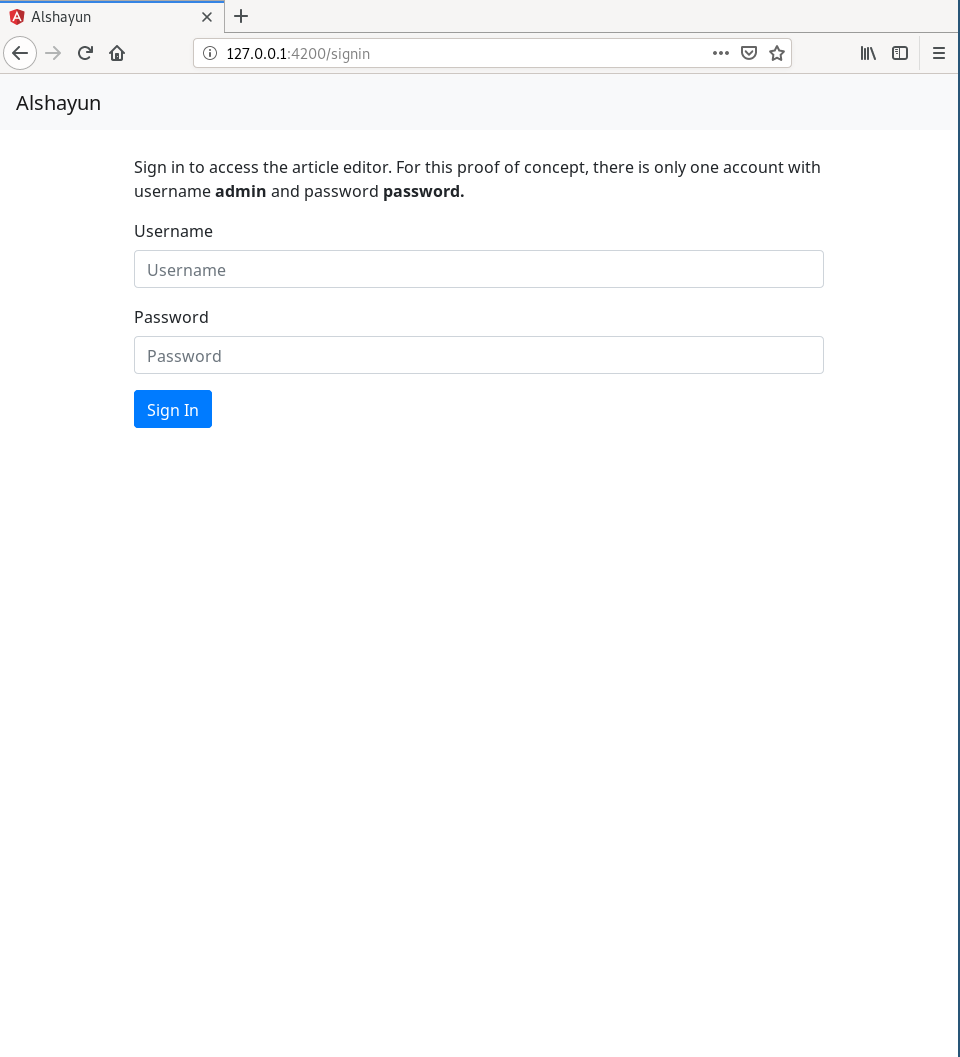
\includegraphics[scale=0.4]{images/qds-login.png}
    \caption{Login page of QDS frontend.}
    \label{fig:qds-login}
\end{figure}

\begin{figure}
    \centering
    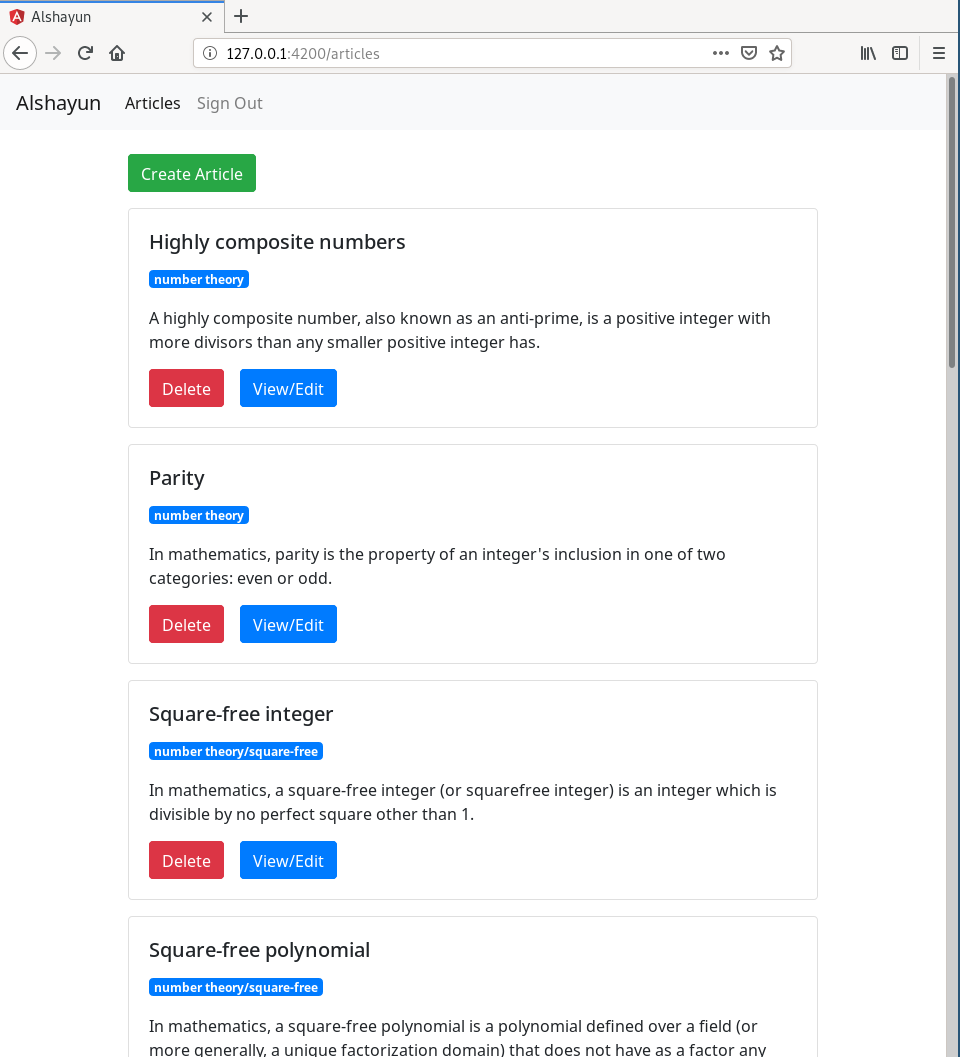
\includegraphics[scale=0.4]{images/qds-articles.png}
    \caption{List of articles in the QDS frontend.}
    \label{fig:qds-articles}
\end{figure}

The user may delete or view and edit an article by clicking the appropriate
buttons next to each article's description. When viewing an article (see Figure
\ref{fig:qds-article}), the user is presented with a field to enter the title of
the article, a field to enter a comma-delimited list of tags associated with the
article, a field to enter a short excerpt of the article, and a field to enter
the main text of the article. Articles are written in Markdown \cite{markdown},
and a live preview of the rendered article is presented next to the editable
article text (see Figures \ref{fig:qds-article}, \ref{fig:qds-create-new}).  The
user may also create a new article by clicking the appropriate button on the
home page.

\begin{figure}
    \centering
    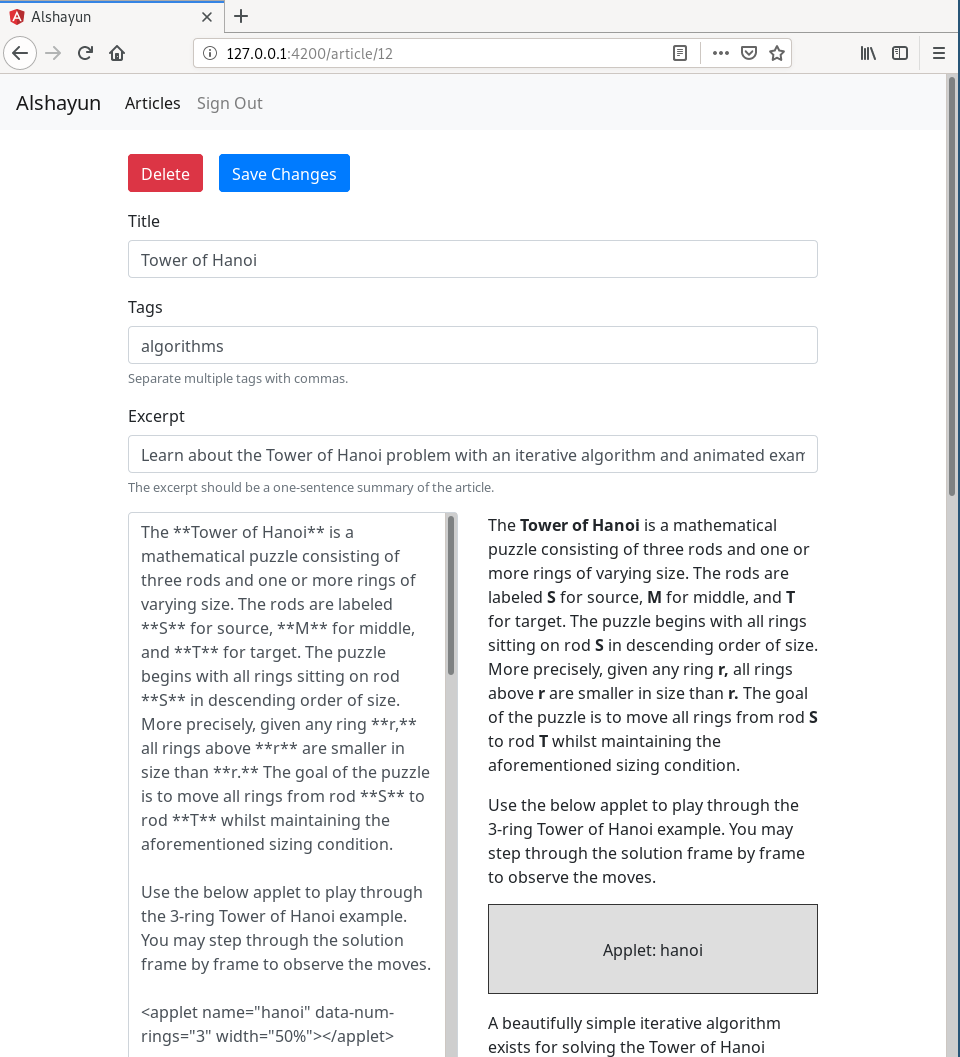
\includegraphics[scale=0.4]{images/qds-article-hanoi.png}
    \caption{Viewing and editing an article in the QDS frontend.}
    \label{fig:qds-article}
\end{figure}

\begin{figure}
    \centering
    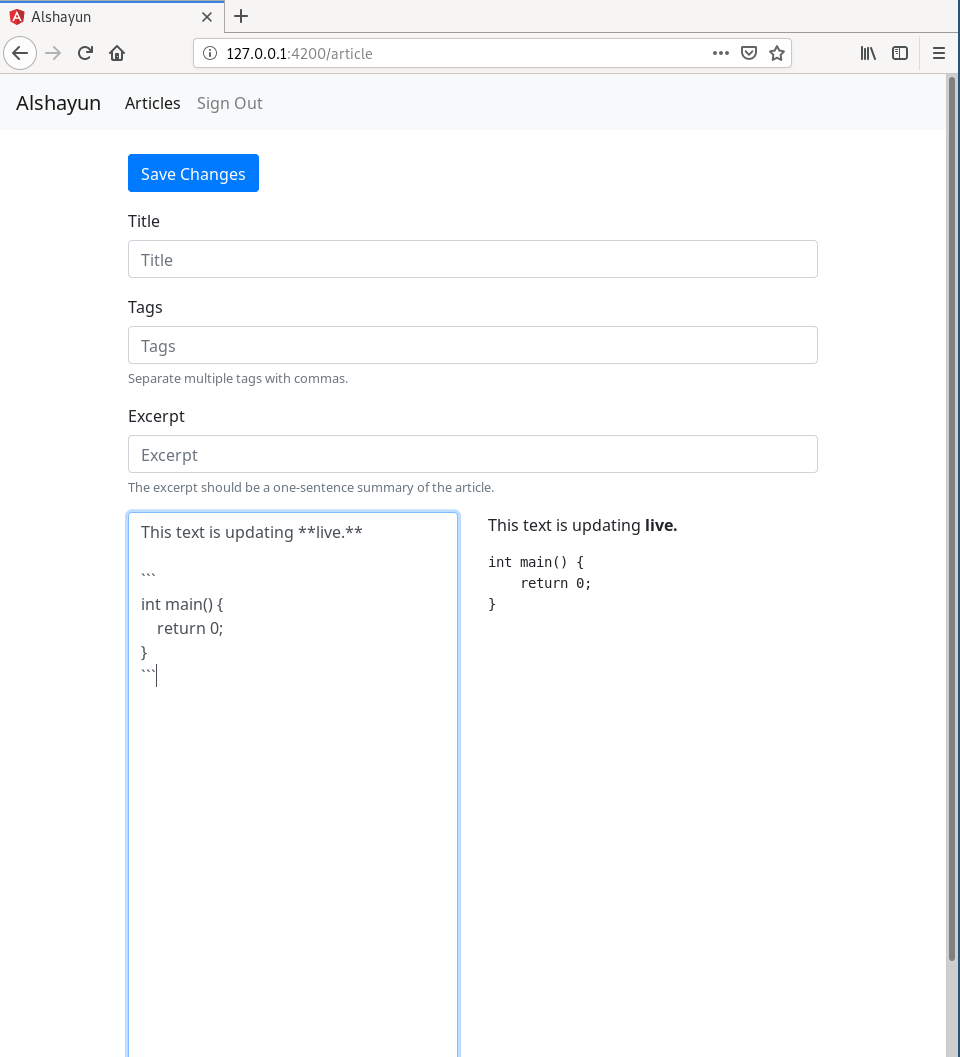
\includegraphics[scale=0.4]{images/qds-create-new.png}
    \caption{Creating a new article in the QDS frontend.}
    \label{fig:qds-create-new}
\end{figure}

    \section{Production Considerations}
    
The \textbf{Flask} instance of the \textbf{backend} runs a built-in development
Web server, as does the \textbf{Angular} instance of the \textbf{frontend}.
However these servers are not designed to handle production scenarios.
Therefore, if an \textbf{Alshayun} user wanted to take the \textbf{QDS} into
production, some things should be taken into consideration first.

For the \textbf{backend}, a real production Web server such as Nginx or Apache
should be setup. The Web server can run a Web Server Gateway Interface (WSGI)
module which redirects applicable requests to the \textbf{Flask} code.
Furthermore, the production Web server can and should have signed Secure Sockets
Layer (SSL) certificates setup to encrypt requests. Lastly, the current
\textbf{backend} has no authentication mechanism for the \textbf{REST}ful
\textbf{API}s exposed to the \textbf{frontend}. Therefore, anyone can
technically create, edit, and delete articles. An authentication mechanism would
need to be developed. Options for this include HTTP Basic Authentication, OAuth,
client certificate authentication handled by the production Web server, or a
variety of other methods.

For the \textbf{frontend}, a real production Web server would also need to be
setup. Perhaps the same Web server powering the \textbf{backend} could be used,
which may help aid in security and latency concerns. SSL certificates and an
administrative account that isn't \texttt{admin/password} is of course
necessary.

\chapter{Alshayun}

    \section{Building and Running}

Building \textbf{Alshayun} requires \textbf{Ionic}, \textbf{Cordova}, and the
Android Software Development Kit (SDK) with all of their dependencies. Note that
while \textbf{Ionic} and \textbf{Cordova} support many platforms, I have only
tested \textbf{Alshayun} with Android, which is why I call it out here. Setting
up such an environment is complicated and time consuming. As a result, I have
built a \textbf{Singularity} container that encapsulates the full development
environment necessary to build and run \textbf{Alshayun.} Using the container is
more complicated than the \textbf{QDS} containers.

To begin, make sure \textbf{Singularity} 3.0 \cite{singularity3inst} or greater
is installed on your computer. I found the container to be useful to all Ionic
developers, so I uploaded it to the Sylabs Cloud Library. To download the image,
run the following command from the application root directory.

\begin{verbatim}
singularity pull ionic.sif library://phphavok/default/ionic:latest
\end{verbatim}

Should that command fail for some reason, or if you prefer to build the
container yourself, run the following command from the application root
directory.

\begin{verbatim}
sudo singularity build ionic.sif Singularity
\end{verbatim}

Once the container has been downloaded or built, run the following commands from
the application root directory.

\begin{verbatim}
mkdir -p sdk/build-tools sdk/platforms
singularity shell \
    -B sdk/build-tools:/usr/local/android/build-tools \
    -B sdk/platforms:/usr/local/android/platforms \
    -p ionic.sif
sdkmanager 'platforms;android-27' 'build-tools;27.0.3'
ionic cordova build android
\end{verbatim}

Note that the \texttt{singularity} command will launch a shell inside the
container environment, and you will still be inside this container environment
upon the completion of the \texttt{ionic} command. You may type \texttt{exit} or
press \texttt{CTRL+D} on your keyboard to exit this environment.

An Android Package (APK) file should be built, which you can install on any
compatible Android device. If you wish to build for a different platform or
version of the Android SDK, you may modify the \texttt{sdkmanager} command as
desired. You can also have \textbf{Ionic} directly install and run the built APK
file on your compatible Android device by attaching your Android device to your
computer via Universal Serial Bus (USB), enabling USB debugging on the Android
device, and running the following command from within the container environment.

\begin{verbatim}
ionic cordova run android
\end{verbatim}

If you don't have an Android device, you may setup and test \textbf{Alshayun} on
an Android Virtual Device (AVD).

        \subsection{Setting up an Android Virtual Device (AVD)}

Exit the container environment and create an additional directory by running the
following command from the application root directory.

\begin{verbatim}
mkdir -p sdk/system-images
\end{verbatim}

Then, once again launch a shell into the container environment, and be sure to
mount in the additional directory.

\begin{verbatim}
singularity shell \
    -B sdk/build-tools:/usr/local/android/build-tools \
    -B sdk/platforms:/usr/local/android/platforms \
    -B sdk/system-images:/usr/local/android/system-images \
    -p ionic.sif
\end{verbatim}

Select a system image to use for your AVD and install it by running the
following command from within the container environment (assuming you chose
Android version 27).

\begin{verbatim}
sdkmanager 'system-images;android-27;google_apis;x86'
\end{verbatim}

Once you've installed a system image, run the following command to list
available devices and pick one.

\begin{verbatim}
avdmanager list devices
\end{verbatim}

After picking a device (\texttt{pixel} in this example), choose a name for your
AVD (e.g., \texttt{test}), and create it using the selected device and system
image installed in the previous steps. Note that, by default, AVDs are installed
under \texttt{\$HOME/.android/avd}. If you want a different path, add \texttt{-p
/path/to/avd} to the \texttt{avdmanager} command.

\begin{verbatim}
avdmanager create avd \
    -n test \
    -k 'system-images;android-27;google_apis;x86' \
    --device pixel
\end{verbatim}

Finally, launch the AVD in an emulator.

\begin{verbatim}
emulator -no-snapshot -avd test
\end{verbatim}

Afterwards, you should be able to install and run APK files on the emulator.

        \subsection{Troubleshooting}

Building may fail if there is not sufficient space in \texttt{/tmp} or under
unpredictable networking circumstances. In the former case, allocate more space
under \texttt{/tmp}. In the latter case, just try the build command again.

    \section{User Interface}
    \section{Caching Strategy}
    \section{Applets}
    \section{Accepting Contributions}

\chapter{Use Cases}
    \section{Classroom Auxiliary Content}
    \section{Starter Mobile Blog}

\chapter{Future Work}
    \section{User Accounts}
    \section{Cloud Hosting}
    \section{Power Efficiency}

\chapter{Conclusion}
    \section{Learning Outcomes}

\begin{thebibliography}{9}
    \bibitem{angular} Angular. Retrieved from \url{https://angular.io/}.
    \bibitem{bootstrap} Bootstrap. Retrieved from
        \url{https://getbootstrap.com/}.
    \bibitem{cordova} Cordova. Retrieved from \url{https://cordova.apache.org/}.
    \bibitem{flask} Flask. Retrieved from \url{http://flask.pocoo.org/}.
    \bibitem{ionic} Ionic. Retrieved from \url{https://ionicframework.com/}.
    \bibitem{markdown} Markdown. Retrieved from
        \url{https://daringfireball.net/projects/markdown/}.
    \bibitem{moore} Moore, Terry. \textit{Why X marks the unknown.} Retrieved
        from \url{https://cosmosmagazine.com/mathematics/why-x-marks-unknown-0}.
    \bibitem{nodejs} Node\@.js. Retrieved from \url{https://nodejs.org/en/}.
    \bibitem{npm} Node Package Manager. Retrieved from \url{https://www.npmjs.com/}.
    \bibitem{pomax} Pomax. \textit{A Primer on Bézier Curves.} Retrieved from
        \url{https://pomax.github.io/bezierinfo/}.
    \bibitem{singularity} Singularity. Retrieved from \url{https://www.sylabs.io/singularity/}.
    \bibitem{singularity3inst} Singularity 3\@.0 Installation Guide. Retrieved
        from
        \url{https://www.sylabs.io/guides/3.0/user-guide/installation.html}.
    \bibitem{typescript} TypeScript. Retrieved from
        \url{https://www.typescriptlang.org/}.
\end{thebibliography}

\end{document}
